\section{Simulation}
Both the yaw and pitch model serve as a good approximation of force, but they do not adequately capture the full dynamics of the EndoWrist.
As mentioned in section \ref{se:est}, having a better description of the general dynamics would allow for state estimates usable for state feedback control \cite{yue2004state}.

State feedback control would allow us to control the force output by the EndoWrist without having the ability to measure it during operation.
Estimated states can be used to calculate the force being applied.
Even though the current models do not allow for useable state estimates of the EndoWrist, in this section the opposite is assumed and simulated on the yaw force model.

As seen in \figref{mdle} our simulation model assumes that the EndoWrist yaw force dynamics consists of the linear system and input nonlinearities identified in chapter \ref{ch:fem}.
Our hypothesis is that full reference following capability can be added to the nonlinear system using only position error measurements and the linear model as part of a Kalman filter.

\begin{figure}[H]
\centering
\includegraphics[width=\textwidth]{simsim.pdf}
\caption{Simulation setup.}
\label{mdle}
\end{figure}

We can see that the outer part of the system consists of a sinusoidal force reference, which is affected by oscillations from the human model. 
This represents the operator's reaction to force feedback while giving a force reference.

The input nonlinearities in the system represent the effects of friction on effort and velocity, as they are the inputs to the plant (EndoWrist).
Only the position error measurement is used as an input to the kalman filter, along with the inputs.

As the Kalman filter outputs the state estimates, they are used for estimating force and providing state feedback to the input.
The estimated force is then sent to the geomagic touch, which transfers it back to the operator.

\begin{figure}[H]
\centering
\hspace{-2.5em}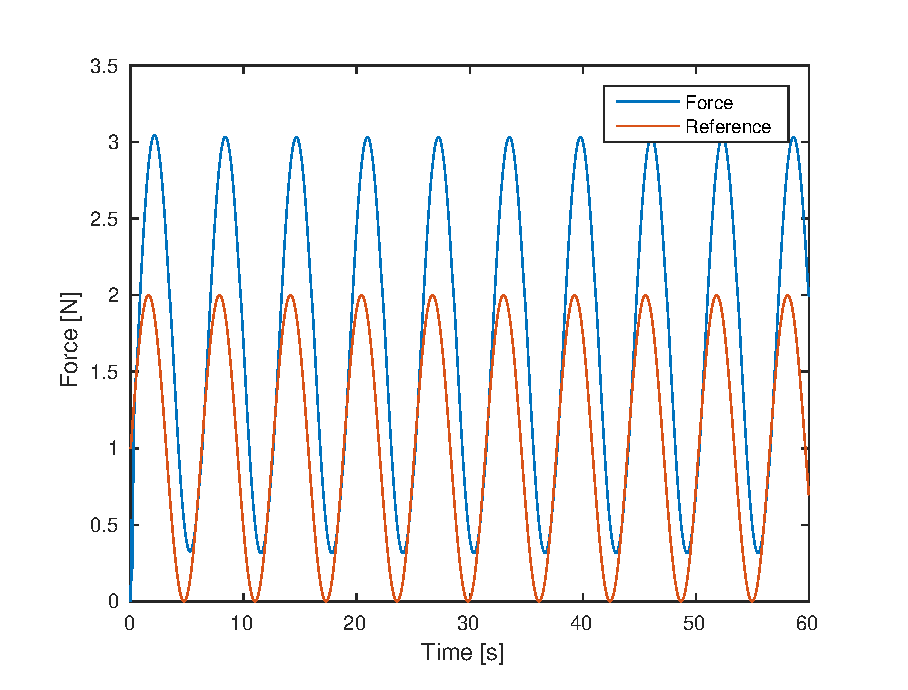
\includegraphics[width=0.7\linewidth]{reference}
\caption{Force reference following.}
\label{fig:freffl}
\end{figure}

As seen in \figref{fig:freffl} the transient behavior of the force matches that of the reference signal.
The offset and amplitude can be corrected by implementing a gain and offset to the reference.

\begin{figure}[H]
\centering
\hspace{-2.5em}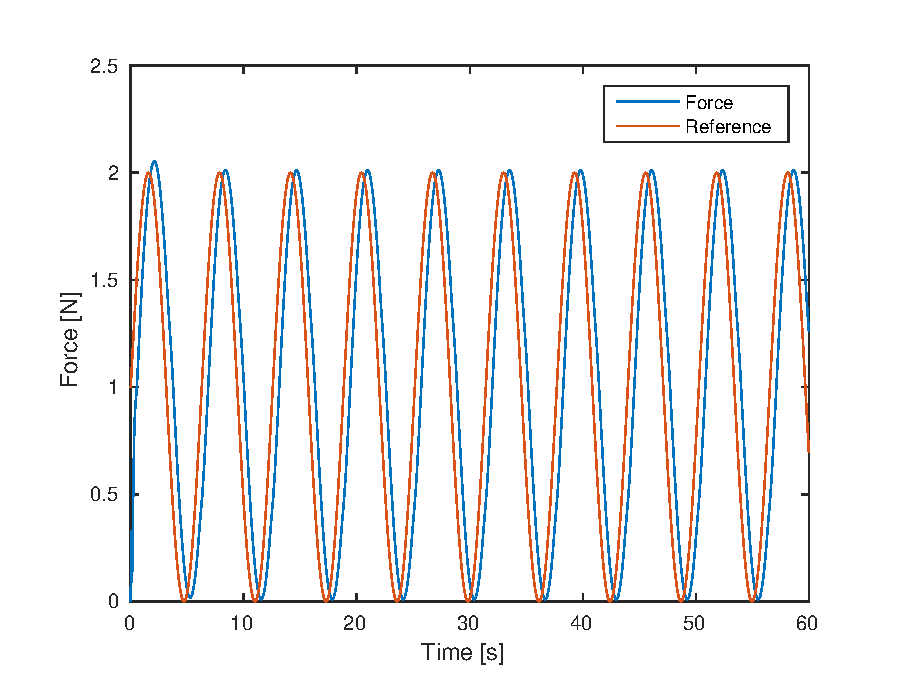
\includegraphics[width=0.7\linewidth]{reference2}
\caption{Force reference following with modified reference.}
\label{fig:freffl2}
\end{figure}

In \figref{fig:freffl2} we can see that the modified reference indeed only leaves a delay in response of the system of about 0.3 seconds.
While this delay is significant in a surgery scenario, we believe it can be further reduced using various state-space methods.